\label{sec:feeding_the_team}

The splitter divides the stream into chunks of data of constant
length, and sends exclusively each chunk to a different \emph{origin
  peer}\footnote{In the route that a chunk follows though the team,
  the origin peer of a chunk is first peer that receives that chunk.},
using a round-robin schema. The teams are created with a least one
peer\footnote{Usually, this peer is a monitor peer (see
  Sec.~\ref{sec:...}), because it can be used by the overlay
  administrator to monitorize the rendering of the stream.} that runs,
by default, in the same host that the splitter and listens to the port
9999. Chunks are enumerated to distinguish them at the peers. More
details about the implementation are available in
Fig.~\ref{fig:chunk_generation}.

%$x$, conforming a message
%$c_x=[x,\text{chunk}]$, where
%$x=i \text{mod} \text{Splitter\_DBS.list\_of\_peers}.\text{length}()$.

\begin{figure*}
  %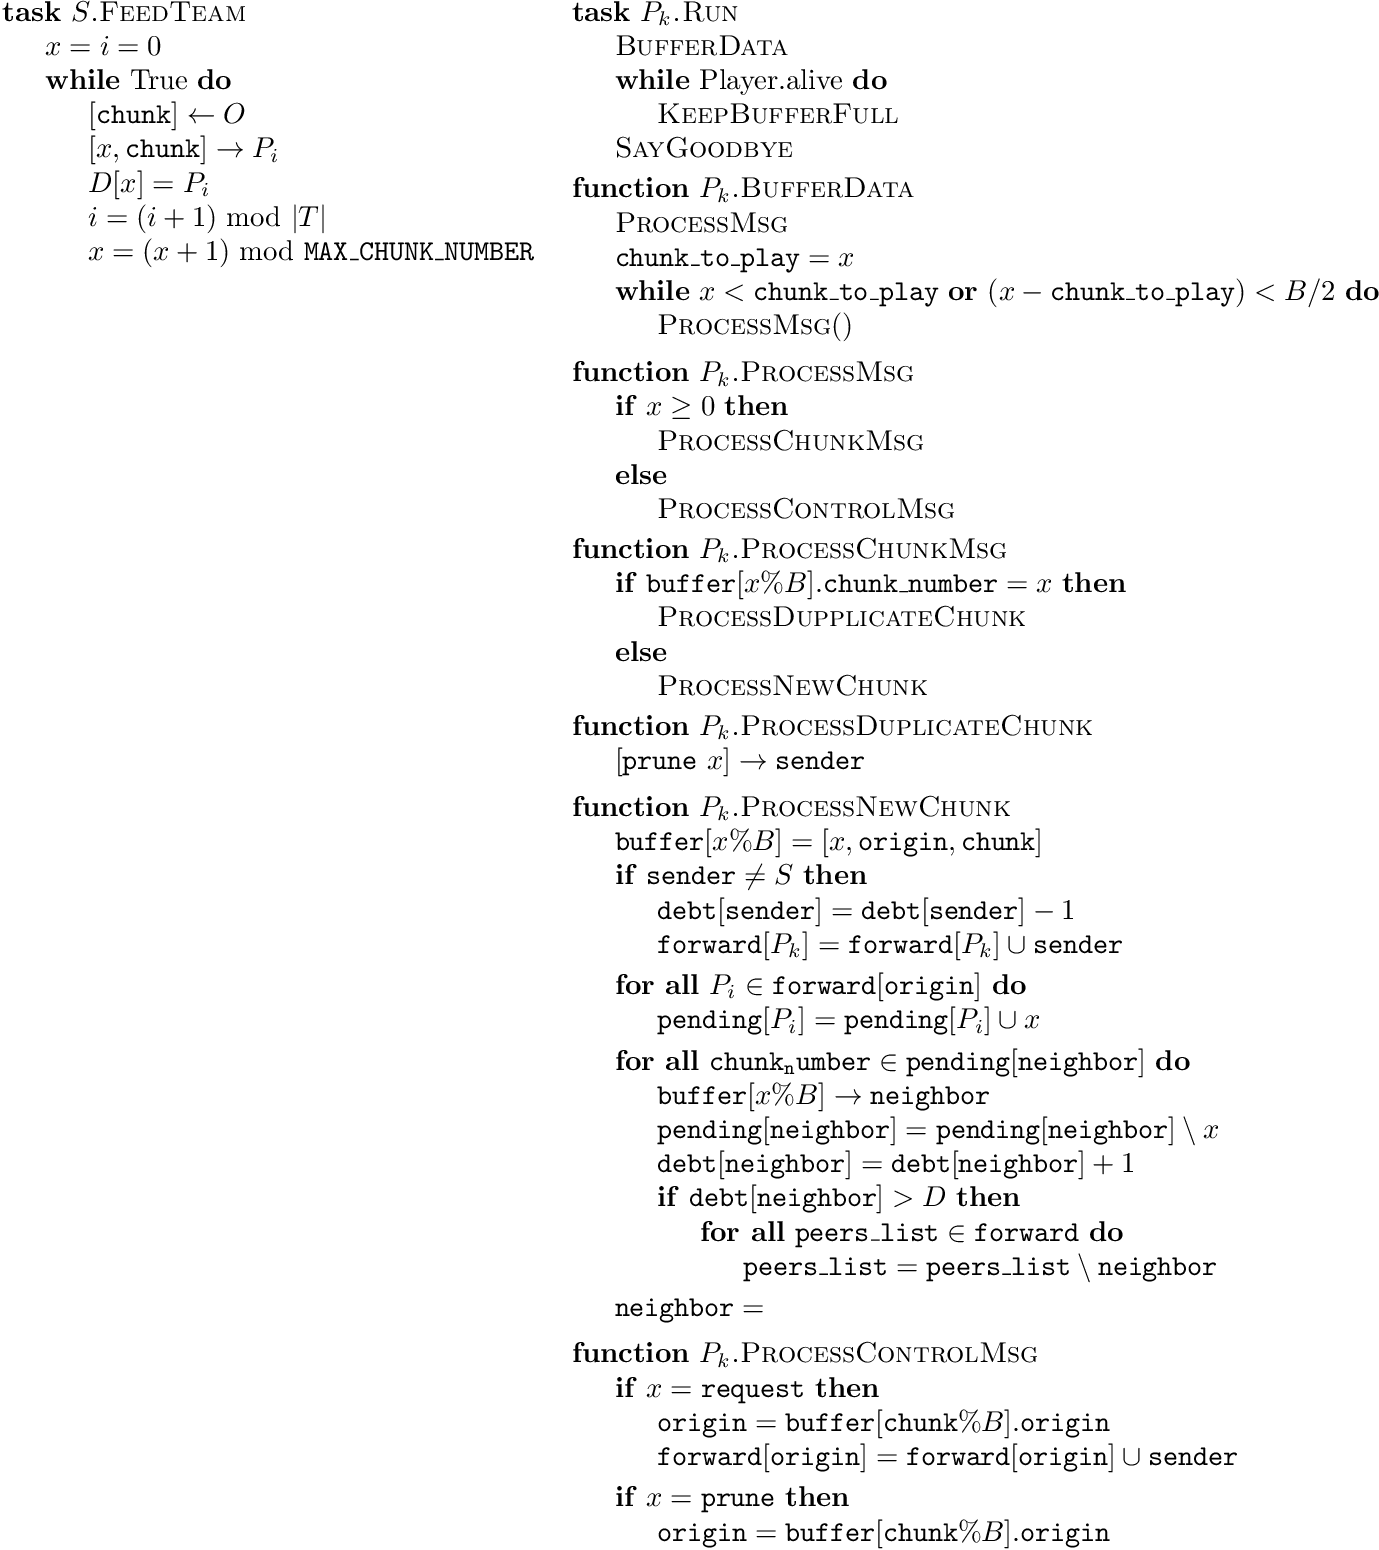
\includegraphics[width=0.75\textwidth]{chunk_generation_and_flooding}
  \fig{300}{3cm}{DBS_splitter_feed} \caption{Chunk
    generation at the splitter and their transmission to the
    team.\label{fig:chunk_generation}}
\end{figure*}

We define a \emph{round} as the process of sending a (different) chunk
from the splitter to the same peer. Notice that the round-time is
variable, and depends on the number of peers in the team, the
chunk-size, and the average bit-rate of the media.

\begin{comment}
(in a team) as the time necessary to send two
consecutive chunks from the splitter (of such team) to the same peer,
using the round-robing. This time is variable and depends on $|T|$,
$C$, and the average bit-rate of the media, $A$.
\end{comment}

\begin{comment}
The round-time is defined by:
\begin{equation}
  \cal{r} = \cal{c}N.
  \label{eq:round_time}
\end{equation}
For example, if we use only one team of $N=256$ peers, a chunk size
$C=1024$~bytes, and a video of $1$~Mb/s, the round time is
\begin{displaymath}
  \cal{r} = \frac{1024\frac{\text{bytes}}{\text{chunk}}\times
    8\frac{\text{bits}}{\text{byte}}}{10^6\frac{\text{bits}}{\text{second}}}\times
  256 \approx 2.1~\text{seconds}.
\end{displaymath}
\end{comment}
